\chapter{\IfLanguageName{dutch}{Stand van zaken}{State of the art}}%
\label{ch:stand-van-zaken}

% Tip: Begin elk hoofdstuk met een paragraaf inleiding die beschrijft hoe
% dit hoofdstuk past binnen het geheel van de bachelorproef. Geef in het
% bijzonder aan wat de link is met het vorige en volgende hoofdstuk.

% Pas na deze inleidende paragraaf komt de eerste sectiehoofding.
\section{Definities}

\begin{itemize}
    \item \textit{Container: Een container is een standaard software-eenheid die code en al zijn afhankelijkheden verpakt, zodat de toepassing snel en betrouwbaar van de ene computeromgeving naar de andere draait \autocite{Docker-2023}. Containers zijn lichtgewicht en bevatten alles wat nodig is om de applicatie te draaien, dus u hoeft niet te vertrouwen op wat er momenteel op de host is geïnstalleerd. \autocite{DockerDocs-2023} }
    \item \textit{Docker: Docker biedt de mogelijkheid om een aplicatie te verpakken en uit te voeren in een geïsoleerde omgeving, genaamd een container.  \autocite{DockerDocs-2023} }
\end{itemize}

Figuur \ref{fig:KubernetesContainers} Geeft een beter beeld wat containers zijn en welke functie docker heeft.

\begin{flushleft}
    \begin{figure}[h]
        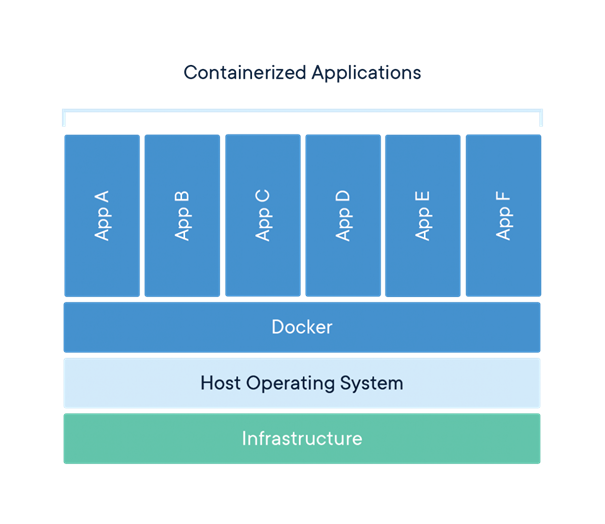
\includegraphics[width=.49\textwidth]{graphics/container.png}
        \caption{\label{fig:KubernetesContainers}Container architectuur \autocite{Docker-2023}}
    \end{figure} 
\end{flushleft}

\section{Kubernetes}
Kubernetes, ook wel afgekort als K8s, is een gratis en open-source systeem dat wordt gebruikt om de implementatie, schaling en het beheer van containerapplicaties te automatiseren \autocite{KubernetesDocs-2023}. 
Het biedt de mogelijkheid om containers die deel uitmaken van een applicatie te groeperen en te beheren als logische eenheden, waardoor het gemakkelijk wordt om deze te beheren \autocite{KubernetesDocs-2023}.
Docker is een containerisatieplatform, terwijl Kubernetes een orkestratietool is voor het beheer van meerdere containers.
Docker biedt een eenvoudige en efficiënte methode voor het aanmaken en inzetten van containers, terwijl Kubernetes complexere functionaliteit biedt voor het beheer van containers op schaal \autocite{banerjee-2023}.
Voor grotere, complexere projecten die uitgebreid containerbeheer vereisen, is Kubernetes een krachtiger en flexibeler hulpmiddel.

\subsection{Kubernetes Componenten - Overview}
\autocite{KubernetesDocs-2023} Bij het ontplooien van kubernetes ontstaat er een cluster. Een cluster bestaat uit een groep machines zogenaamd \textit{worker nodes}. Zo een node heeft verschillende componenten zoals een Kubelet, een kube-proxy en een container-runtime.
Binnen deze worker nodes zijn er pods met containers in. In deze containers kunnen applicaties zoals een SQL database of een website draaien. 
\autocite{KubernetesDocs-2023} Binnen een cluster is er ook een control plane die de globale beslissingen neemt over bijvoorbeeld scheduling of een pod starten. De control plane beheert ook de nodes. 
\autocite{KubernetesDocs-2023} Een control plane bestaat uit verschillende componenten zoals een Kube-apiserver, etcd, kube-scheduler en een kube-controller-manager. 
De kube-apiserver is een belangrijk component van de control plane want deze is verantwoordelijk voor de communicatie van gebruikers, de cluster en externe componenten \autocite{hohn-2020}. 
De kubernetes API laat toe om de staat van objecten zoals pods, namespaces te manipuleren \autocite{KubernetesDocs-2023}.
De etcd binnen een control plane is een key value opslagplaats voor alle data van de cluster, het is belangrijk dat ten alle tijde deze data beschermd is van ongewilde manipulatie \autocite{KubernetesDocs-2023}. 
Om voor fouttolerantie en hoge beschikbaarheid te zorgen, draait de control plane in productiescenario's meestal op vele machines, en een cluster bevat doorgaans meerdere nodes \autocite{KubernetesDocs-2023}. 
In leer- of middelenbeperkte omgevingen is er meestal maar één node aanwezig.

\subsubsection{pod}
Een pod is een groep van één of meer containers \autocite{habbal-2020}.
Alle containers in een pod delen hetzelfde IP adres en dezelfde middelen zoals volumes \autocite{hohn-2020}.
In makkelijkere woorden is een pod een enkele instantie van een applicatie die kan worden gerepliceerd als er meer instanties nodig zijn om de toenemende druk op te vangen \autocite{habbal-2020}.
Gerepliceerde pods worden gecreëerd en beheert als een groep door de middelen en de control plane \textcite{KubernetesDocs-2023}.

\subsubsection{Service}
\textit{Een service is een methode om een netwerktoepassing die als een of meer Pods in uw cluster draait, bloot te stellen \autocite{KubernetesDocs-2023}.}

\subsubsection{Namespace}
Een namespace dient om objecten te organiseren in een cluster.
Een soort folder die objecten houd \autocite{burns-2022}.

\subsubsection{Kubelet}
De kubelet is het belangrijkste component dat op elke node aanwezig is \autocite{Vayghan2019}.
Kubelet draait de Docker-containers die aan zijn node zijn toegewezen, voert regelmatig gezondheidscontroles op ze uit, en rapporteert hun status en die van de node aan de master \autocite{Vayghan2019}.

\subsubsection{Volume}
Een volume maakt het mogelijk om opslag te delen tussen de containers in een pod, of tussen pods op dezelfde node \autocite{Baier2017}.

\subsubsection{ConfigMap}
De ConfigMap binnen kubernetes is een soort volume en een middel voor het opslaan van configuratie data \autocite{KubernetesDocs-2023}.
Het is een manier om configuratie data te injecteren in pods \autocite{KubernetesDocs-2023}.

\subsubsection{Kubectl}
Kubectl is een commmand-line tool om opdrachten, ook wel commando's genoemd, te kunnen uitvoeren op de control plane van de cluster.
Deze command-line tool maakt gebruik van de Kubernetes API \autocite{KubernetesDocs-2023}.

\begin{flushleft}
    \begin{figure}[h]
        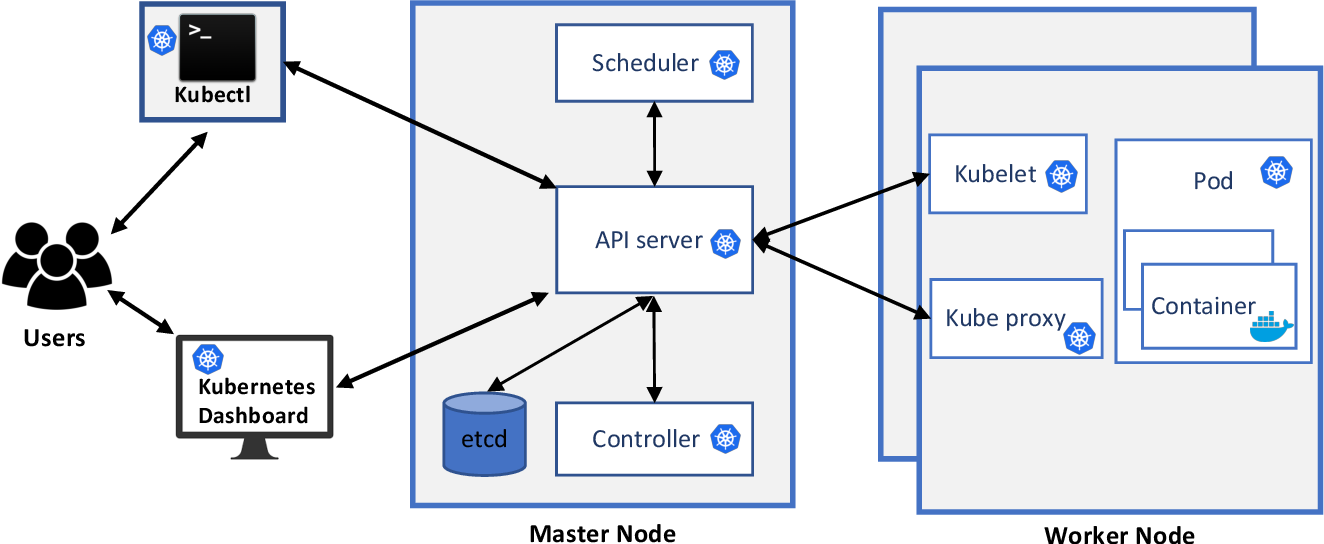
\includegraphics[width=.70\textwidth]{graphics/3-Figure1-1.png}
        \caption{\label{fig:KubernetesOverview}Deze afbeelding geeft een duidelijk overzicht van de componenten van kubernetes en hoe ze met elkaar interacteren.  \autocite{shamim2020xi}}
    \end{figure} 
\end{flushleft}


\section{Kwetsbaarheden}

\subsection{Misconfiguratie}
Een studie in 2023 van \textcite{red-hat-2023} toont aan dat 45 percent van DevOps ingenieurs een veiligheidsincident heeft ervaren die te maken heeft met de misconfiguratie van containers en/of clusters. Pods in een Kubernetes-cluster kunnen standaard met elkaar communiceren, door deze communicatie ontstaan er veiligheidslekken als het niet goed is geconfigureerd. De grootste bezorgdheid rond misconfiguratie is het blootstellen van gevoelige informatie \autocite{red-hat-2023}. Andere soorten veiligheids misconfiguraties dat de ingenieurs zich zorgen om maken zijn ongepatchte fouten, het behoud van de standaard configuratie, errors in de code en containers met foute rechten. \newline

Vaak voorkomende misconfiguratie fouten kunnen tot grote problemen voor een applicatie zorgen. Namelijk 40 percent zijn het meest bezorgd dat er ransomware aanvallen gebeuren als kubernetes of de containers niet juist zijn geconfigureerd en 53 percent hebben al een ransomware aanval ervaren in de laatste 12 maanden \autocite{red-hat-2023}. De meest voorkomende aanval bij misconfiguraties is een Denial of service (DoS) attack \autocite{red-hat-2023}. Een DoS aanval heeft als doel het systeem onbruikbaar of ontoegankelijk te maken voor de gebruikers. \newline

Standaard configuratie binnen de kubernetes cluster kan leiden tot anonieme niet-geauthenticeerde gebruikers om kwaadaardige activiteiten uit te voeren. Een kwaadwillende gebruiker kan bijvoorbeeld de standaardinstellingen voor een onbeveiligde toegang achterhalen, toegang krijgen tot de control plane en schadelijke commando's uitvoeren \autocite{shamim2020xi}.

\subsection{API server}
Via de kubectl command is het mogelijk om API requests naar de server te sturen om middelen en workloads te beheren \autocite{KubernetesDocs-2023}. Iedereen die schrijf rechten heeft of iedereen die toegang heeft tot de Kubernetes API kan de cluster controleren \autocite{KubernetesDocs-2023}. 
Standaard zal de API server luisteren naar poort 6443 \autocite{KubernetesDocs-2023}. Iedereen die toegang krijgt tot het systeem waar de master op draait, heeft volledige toegang tot de cluster \autocite{Rice2018}. \newline

\subsection{RBAC}
RBAC (Rolgebaseerde toegangscontrole) is het concept dat machtigingen worden geassocieerd met rollen, en dat gebruikers lid worden van de juiste rollen, waardoor zij de machtigingen van de rollen verkrijgen \autocite{Sandhu1998}. Doordat misconfiguraties niet vanaf een centrale locatie kunnen worden gedetecteerd, hersteld en voorkomen, kunnen clusters worden gecompromitteerd \autocite{OWASP-2023}. Volgens de top 10 Kubernetes risico's van OWASP in 2022 is RBAC de derde meest gevaarlijke risico. RBAC is de primaire authorisatie methode voor Kubernetes en is verantwoordelijk van de permissies over de middelen en componenten \autocite{OWASP-2023}. Er bestaat een 'superuser' binnen kubernetes genaamd cluster-admin. Deze cluster-admin heeft toegang om elke actie uit te voeren op elke component binnen een Kubernetes cluster \autocite{OWASP-2023}. 

RBAC wordt gebruikt om elk verzoek dat binnenkomt op de API-server goed te keuren of te weigeren \autocite{mytilinakis2020attack}. Als een gebruiker een API request maakt naar het eindpunt zonder enige authenticatie dan is hij geassocieerd met als een anonieme gebruiker \autocite{mytilinakis2020attack}. Het mogelijk maken van anonieme toegang naar eindpunten kan ook de waarschijnlijkheid van het vrijgeven van gevoelige informatie verhogen \autocite{Rice2018}. Het is onwaarschijnlijk dat deze informatie iets belangrijks in gevaar brengt, maar het kan de aanvaller de weg wijzen naar andere zwakheden \autocite{Rice2018}.

\subsection{Software Supply chain}
35 percent van de respondenten in de studie van \textcite{red-hat-2023} zijn het meest bezorgd over kwetsbaarheden in de software gerelateerd aan de software supply chain. Een software supply chain is de verzameling van de componenten, softwares, tools die gebruikt worden om een applicatie te bouwen. Hierbij komen open-source softwares aanbod en het gebruik hiervan creëren uitdagingen in de beveiliging van de applicatie \autocite{red-hat-2023}. Kwetsbaarheden in software kunnen leiden tot grote beveiligingsproblemen, zoals datalekken, malware-infecties en onbevoegde toegang \autocite{shamim2020xi}. De bedrijven van de correspondenten zijn het meest bezorgd in kwetsbare componenten van een applicatie, onvoldoende toegang controle en een tekort aan Software Bill of Materials (SBOM) of herkomst \autocite{red-hat-2023}. Deze studie toont ook aan dat bijna 70 percent van de correspondenten al problemen hebben gehad met een kwetsbare CI/CD pipeline en kwetsbare componenten in de applicatie. \newline

Containers en docker images horen ook tot software supply chain. Containers kunnen kwetsbaarheden en schadelijke software bevatten. Als er zwakheden in een Kubernetes-cluster zitten, wordt het hele container-orkestratiesysteem, evenals de meegeleverde apps, kwetsbaar voor aanvallen \autocite{shamim2020xi}. Als de images en deployment-configuraties van Kubernetes-componenten niet worden gecontroleerd, kan het Kubernetes-cluster vatbaar worden voor onbevoegde gebruikers. Wanneer deze images worden uitgerold, kunnen aanvallers toegang krijgen en gebruikmaken van zwakke plekken \autocite{shamim2020xi}. \newline

Volgens \textcite{OWASP-2023} zijn er drie belangrijke termen binnen de kwetsbaarheden van supply chain:
\begin{itemize}
    \item Image Integrity: Dit verwijst naar de zekerheid van een container image. De zekerheid dat de image is wat het beweert te zijn, dat het geen kwaadaardige code bevat en dat het in geen enkele wijze aangepast is \autocite{OWASP-2023}. 
    \item Image Composition: Een container image is opgemaakt uit verschillende lagen. Elke laag representeert bepaalde veiligheidsimplicaties. Container images met onbelangrijke software kunnen gebruikt worden om privileges te verhogen of kwetsbaarheden uit te buiten \autocite{OWASP-2023}. 
    \item Bekende software kwetsbaarheden: Vele container images gebruiken paketten van derde partijen die kwetsbaarheden kunnen bevatten die uitgebuit kunnen worden. Als docker images kwetsbare versies van software bevatten kan dit de kubernetes cluster in gevaar brengen \autocite{OWASP-2023}. 
\end{itemize}


\subsection{Container runtime}
In het onderzoek van \textcite{red-hat-2023} toont aan dat 49 percent van de gerelateerde veiligheidsincidenten in kubernetes of containers gebeuren via beveiligingsincidenten tijdens runtime. De container runtime is een van de meest kritische componenten in een kubernetes cluster \autocite{mytilinakis2020attack}. De container runtime dat in dit onderzoek wordt gebruikt is Docker, de meest voorkomende. Docker heeft zelf veiligheidsinstellingen en functies. Kwetsbaarheden in containers kunnen leiden tot het in gevaar brengen van andere componenten. 

\subsection{Images}
In de sectie van \textit{Software supply chain} wordt er al een klein stukje besproken over images. Images worden meestal uit een publieke plaats gedownload. Het is dus mogelijk dat deze docker images niet altijd de juiste intenties hebben en mogelijks kwade bedoelingen hebben en kwetsbaarheden veroorzaken \autocite{mytilinakis2020attack}. 

\subsection{Kubernetes API server}
\paragraph{Statische pods}
Volgens \textcite{KubernetesDocs-2023} is er een risico bij statische pods waarbij aanvallers statische pods kunnen wijzigen of nieuwe statische pods kunnen toevoegen waardoor API-serverconroles worden omzeild. 
Dit risco kan worden veroorzaakt door foute schrijfrechten toe te kennen tot de locatie waar statische pods zijn opgeslagen.

\paragraph{Kubelet API}
De kubelet API biedt een HTTP API dat informatie vrijgeeft over de draaiende pods, pod logs en staat het uitvoeren van commando's in containers toe.
Directe toegang tot de Kubelet API maakt het mogelijk om die informatie openbaar te maken. \autocite{KubernetesDocs-2023}.
Rechtstreekse toegang valt niet onder toelatingscontrole en er wordt geen logging gemaakt door Kubernetes audit logging. Een aanvaller met directe toegang tot deze API kan mogelijk controles omzeilen die bepaalde acties detecteren of voorkomen \autocite{KubernetesDocs-2023}.

\paragraph{The etcd API}
De etcd service wordt gebruikt als dataopslag voor Kubernetes. Onbevoegde toegang tot deze API maakt openbaring of aanpassing van een cluster \autocite{KubernetesDocs-2023}. Rechtstreekse toegang tot de etcd wordt niet gelogd door de audit.
Een aanvaller met toegang tot de private sleutel van het etcd-clientcertificaat van de API-server of een vertrouwd clientcertificaat kan clusterbeheerdersrechten krijgen \autocite{KubernetesDocs-2023}. Fout geconfigureerde etcd instellingen kunnen de database open zetten tot aanvallen van buitenaf en ongewilde toegang \autocite{KubernetesDocs-2023}.

\paragraph{Container runtime socket}
Toegang tot de runtime socker container maakt het mogelijk om nieuwe containers op te zetten of te interageren met actieve containers. Indien gecompromitteerd, kan een aanvaller privileges escaleren, toegang krijgen tot geheimen en andere worker nodes of control plane componenten controleren \autocite{KubernetesDocs-2023}.

\section{Tools en oplossingen}

\subsection{misconfiguratie}
Deze sectie bespreekt algemeen advies hoe de configuratie kan verbetert worden en bespreekt ook verschillende tools voor het verifiëren van de configuratie.\newline

Om beveiliging in te stellen op een pod kan dit met het veld \textit{securityContext} in de specificatie van de pod. \textit{securityContext} is een \textit{PodSecurityContext} object \autocite{KubernetesDocs-2023}. 
Deze beveiligingsinstellingen gelden voor alle containers binnen de pod \autocite{KubernetesDocs-2023}. 
Volgens \textcite{OWASP-2023} is een proces als root gebruiker draaien een vaak voorkomende fout. Voor sommige workloads is de root gebruiker een vereiste maar het is aangeraden om het te vermijden. Als de container met root rechten gecompromitteerd wordt dan zou de aanvaller root rechten hebben om schadelijke acties te kunnen uitvoeren \autocite{OWASP-2023}.  \newline

Een ander voorbeeld van \textcite{OWASP-2023} beschrijft dat het aangeraden is om read-only (alleen-lees) bestandssystemen te gebruiken. Alleen-lees bestandssystemen limiteren de impact van een gecompromitteerde container op een kubernetes node \autocite{OWASP-2023}. Dit zorgt ervoor dat een kwaadaardig proces het host systeem niet kan herschrijven of aanpassen. Volgens \textcite{OWASP-2023} is het aangeraden om containers zonder privileges te draaien. De container kan verdere middelen of capaciteiten krijgen als de container als privilege draait. \newline

Deze drie voorbeelden kunnen allemaal vermeden worden in de configuratie van een pod. Dit is bij de sectie 'securitycontext'. 
\begin{lstlisting}
apiVersion: v1  
kind: Pod  
metadata:  
    name: root-priviliged-readOnly
spec:  
    containers:  
    ...
    securityContext:  
        #Privileges staan aan 
        privileged: true
        #root gebruiker staat aan
        runAsUser: 0
        #De container runned als een gebruiker en niet als root
        runAsUser: 5554
        #alleen-lees rechten zijn geconfigureerd
        readOnlyRootFilesystem: true
\end{lstlisting}


Het is ook mogelijk om dit als runtime te configureren en niet in de configuratie. De applicatie kan deze miconfiguratie mitigeren door volgende maatregelen te nemen \autocite{OWASP-2023}:
\begin{itemize}
    \item Draai als niet-root gebruiker: Standaard draaien containers in Kubernetes als de root-gebruiker, die onbeperkte toegang heeft tot het systeem. Het draaien van containers als een niet-rootgebruiker kan de impact van potentiële beveiligingskwetsbaarheden helpen beperken door het niveau van toegang dat de container heeft tot het onderliggende systeem te verlagen \autocite{OWASP-2023}.
    \item Uitvoeren als niet-privilege modus: Standaard hebben containers in Kubernetes geprivilegieerde toegang tot het hostsysteem, wat betekent dat ze acties kunnen uitvoeren die de beveiliging van het systeem in gevaar kunnen brengen. Het draaien van containers in niet-privilege modus kan dit helpen voorkomen door de acties die de container kan uitvoeren te beperken \autocite{OWASP-2023}.
    \item Stel AllowPrivilegeEscalation op \textit{False}: Deze instelling verbiedt dat kindprocessen meer privileges krijgen dan hun ouderprocessen. Het voorkomt de escalatie van privileges binnen de container, wat beveiligingsproblemen kan helpen voorkomen \autocite{OWASP-2023}.
\end{itemize}

\subsubsection{Toegang tot Kubernetes API}
Kubectl maakt contact met de API server via REST calls. Bij zo een REST call naar de API, gaat de API door verschillende stadia \autocite{KubernetesDocs-2023}: 
\begin{itemize}
    \item Transport beveiliging
    \item Authenticatie
    \item Autorisatie
    \item Toegangscontrole
\end{itemize}
\paragraph{Transport beveiliging}
Het is belangrijk dat de API server niet naar een poort luistert die kwetsbaar is zoals poort 8080. Volgens \autocite{KubernetesDocs-2023} is de standaard poort 6443. Om zeker te zijn is het mogelijk om te checken op welke poort de API server draait door het commando:
\begin{lstlisting}[language=tex, caption={Checken welke poort de API server draait}]
kubectl config view --minify -o jsonpath='{.clusters[0].cluster.server}'
\end{lstlisting}

De API is veilig geconfigureerd als de URL eindigt met poort 443, 8443 of 6443. Het aangeraden om dit te veranderen naar poort 6443, 8443 of 443 als de poort geconfigureerd is op 8080. Dit is mogelijk met het commando:
\begin{lstlisting}[language=tex, caption={Veranderen poort Kubernetes API}]
kube-apiserver --secure-port <port>
\end{lstlisting}

Om bovenstaand commando uit te voeren is het nodig om kube-apiserver te installeren. 
Bovenstaand commando zal de URL geven van de kubernetes API sever. Om te verifiëren dat de poort open is kan dat met een curl commando \autocite{Rice2018}:
\begin{lstlisting}[language=tex, caption={verifiëren poort open}]
curl <IP address>:<port>
\end{lstlisting}

Bij het maken van een API verzoek of REST call wordt er ook een certificaat gepresenteerd. Zo een certificaat kan ondertekent zijn door een certificate authority (CA) of een PKI (public key infrastructure) die connectie heeft met een gekende CA. Het certificaat en de private sleutel kunnen gewijzigd worden door gebruik te maken van volgende commando's \autocite{KubernetesDocs-2023}:
\begin{lstlisting}[language=tex, caption={Wijzigen certificaat en private sleutel}]
kube-apiserver --tsl-cert-file
kube-apiserver --tls-private-key-file
\end{lstlisting}

\paragraph{Authenticatie}
Eens dat er een veilige transport methode is toegepast kijkt de API naar authenticatie. Authenticatie kan plaatsvinden via clientcertificaten, wachtwoorden, tokens, serviceaccounts. Meerdere authenticatiemethoden kunnen worden ingesteld en geprobeerd.
Als een API verzoek niet kan worden geauthenticeerd dan is het verzoek geweigerd met de HTTP status code 401 \autocite{KubernetesDocs-2023}.  

\paragraph{Autorisatie}
Geauthenticeerde verzoeken moeten worden geautoriseerd. Een verzoek moet een gebruikersnaam, actie en object van de actie bevatten. Het verzoek is geautoriseerd als het niet wordt geweigerd en de gebruiker toegang heeft om die actie uit te voeren \autocite{KubernetesDocs-2023}.
Kubernetes maakt gebruik van meerdere authorisatiemethodes zoals ABAC, RBAC en Webhook mode \autocite{KubernetesDocs-2023}. 

\paragraph{Toegangscontrole}
Toegangscontrolemodules kunnen verzoeken wijzigen of weigeren. Toegangscontrolemodules zijn softwaremodules die verzoeken kunnen wijzigen of weigeren. Deze modules   handelen verzoeken af die objecten creëren, wijzigen, verwijderen of verbinden. 

\subsubsection{Kubernetes API server}
In de sectie \textit{kwetsbaarheden} worden 4 delen van de Kubernetes API server aangehaald met hun kwetsbaarheden. In deze sectie wordt er beschreven hoe deze kwetsbaarheden gemitigeerd kunnen worden.

\paragraph{Statische pods}
De oplossingen die \textcite{KubernetesDocs-2023} biedt zijn:
\begin{itemize}
    \item Gepaste permissies instellen voor toegang tot de configuratie file van Kubernetes \textit{/etc/kubernetes/kubelet.conf} 
    \item Schakel de \textit{kubelet static pod manifest} functionaliteit alleen in als de node dit vereist: Bewerk het kubelet-configuratiebestand (bijvoorbeeld /etc/kubernetes/kubelet.conf) en stel \textit{staticPodPath} of \textit{staticPodURLs} in op basis van de vereisten.
\end{itemize}

\paragraph{De kubelet API}
De oplossingen die \textcite{KubernetesDocs-2023} bied voor het mitigeren van de kwetsbaarheden in de kubelet API zijn:
\begin{itemize}
    \item Beperk de toegang tot subbronnen van het API object door middel van technieken zoals RBAC. Geef alleen toegang wanneer het nodig is.
    \item Beperk de toegang tot de kubelet poort
    \item Configureer kubelet authenticatie om webhook of certificaat modus te gebruiken: Bewerk het kubelet-configuratiebestand (bijv. /etc/kubernetes/kubelet.conf) en stel de authenticatiemodus in op webhook of certificaat op basis van de kubernetes opstelling
    \item Schakel de niet-geauthenticeerde alleen-lezen Kubelet-poort op het cluster uit: Bewerk het kubelet-configuratiebestand (bijv. /etc/kubernetes/kubelet.conf) en stel readOnlyPort: 0 in om de alleen-lezen poort uit te schakelen.
\end{itemize}

Een oplossing die \textcite{OWASP-2023} biedt is om de optie \textit{--anonymous-auth} op false te zetten in de kubelet configuratie zodat er geen anonieme authenticatiemogelijkheden zijn tot de kubelet API.

\paragraph{etcd API}
De oplossingen die \textcite{KubernetesDocs-2023} bied voor het mitigeren van de kwetsbaarheden in de etcd API zijn:
\begin{itemize}
    \item Zet de gepaste bestandspermissies voor de bestanden van de private sleutel aan de hand van volgend commando:
\begin{lstlisting}[language=tex, caption={Opzetten gepaste bestandspermissies voor private sleutel}]
chmod <permissions> <private_key_file>
\end{lstlisting}
    \item Zorg ervoor dat de certificaat autoriteit die vertrouwd is door de etcd alleen gebruikt word voor de authenticatie van die dienst. 
    \item Beperk toegang tot de etcd poort via het netwerk
\end{itemize}

\paragraph{Container runtime socket}
De oplossingen die \textcite{KubernetesDocs-2023} bied voor het mitigeren van de kwetsbaarheden in container runtime socket zijn:
\begin{itemize}
    \item Stel de juiste bestandsrechten in voor het container runtime socket bestand:
\begin{lstlisting}[language=tex, caption={Opzetten juiste bestandsrechten voor container runtime socket}]
chmod <permissions> <container_runtime_socket>
\end{lstlisting}
    \item Isoleer de kubelet van andere componenten die op het node draaien, met behulp van technieken als Linux kernel namespaces.
    \item Beperk of verbied het gebruik van hostPath mounts die de container runtime socket bevatten.
\end{itemize}

\subsubsection{Beveiligingsstandaarden pod}
\paragraph{Beleidsregels}
\textcite{KubernetesDocs-2023} beschrijft 3 beleidsregels: geprivilegieerd, basislijn en beperkt. Deze beleidsregels zijn cumulatief en varieren van sterk toelaatbaar tot sterk beperkend. 

\paragraph{Geprivilegieerd}
\textit{Het beleid van de privileges is met opzet open en volledig onbeperkt. \autocite{KubernetesDocs-2023}}.
Deze beleidsregel is bestemd voor gebruikers die vertrouwd zijn voor het beheer van het syteem en de infrastructuur \autocite{KubernetesDocs-2023}. 

\paragraph{Basislijn of Basisbeleid (Baseline)}
\textit{Het basisbeleid is gericht op gebruiksgemak voor gewone gecontaineriseerde werklasten, terwijl bekende privilege-escalaties worden voorkomen. \autocite{KubernetesDocs-2023}}
Deze beleidsregel is bestemd voor applicatiebeheerders en -ontwikkelaars van non-kritische applicaties.
In de officiële documentatie van Kubernetes zijn de exacte controls en beleidsregels te vinden.

\paragraph{Beperkt}
\textit{Het beperkte beleid is gericht op het afdwingen van de huidige Pod hardening best practices, ten koste van enige compatibiliteit. \autocite{KubernetesDocs-2023}}
Deze beleidsregel is gericht naar applicaties die beveiligingskritisch zijn en alleen vertrouwde gebruikers. 
Dit beperkt beleid bevat dezelfde controles als het basisbeleid maar worden strikter toegepast.

\subsubsection{Tools of middelen misconfiguratie}


\subsection{RBAC}
RBAC (Role-based access control) of rolgebaseerde toegangscontrole wordt gebruikt om toegang te controleren voor gebruikers en werklasten \autocite{nordell2022systematic}.
Zo hebben gebruikers en werklasten alleen toegang tot de middelen die nodig zijn om hun rollen uit te voeren.

\subsubsection{Best practices}
\textcite{KubernetesDocs-2023} en \textcite{OWASP-2023} beschrijven een aantal generieke regels die van toepassing zijn bij RBAC in een kubernetes cluster:
\begin{itemize}
    \item Gebruik rechten op het niveau van namespace
    \item Gebruik RoleBindings in de plaats van ClusterRoleBindings om gebruikers alleen rechten te geven binnen een specifieke namespace
    \item Least-privilege rechten toekennen
    \item Ontwijk wildcard permissies
    \item Limiteer het gebruik van 'cluster-admin' accounts
    \item Zet een gecentraliseerd beleid in om riskante RBAC-machtigingen op te sporen en te blokkeren
\end{itemize}

Het belangrijkste beveiligingsprobleem binnen RBAC is het ongeautoriseerde gebruik van tokens  \autocite{nordell2022systematic}.  \textcite{KubernetesDocs-2023} raadt aan om de distributie van tokens te minimaliseren en het aantal nodes die krachtige pods draaien te limiteren. Als er zich krachtige pods plaatsvinden in de cluster is het belangrijk dat deze niet naast andere krachtige pods begeven. 

\subsubsection{Tools of middelen RBAC}


\subsection{Software Supply Chain}
De studie van \textcite{ellison2010evaluating} beschrijft dat het reduceren van de aanvalsoppervlak (of attack surface) helpt bij het beveiligen van de supply chain. Een systeem met een groter aantal te exploiteren componenten heeft een groter aanvalsoppervlak en loopt een groter risico op gevaar voor exploitatie \autocite{ellison2010evaluating}. Vermijd daardoor onnodige software. Enkele methoden die \textcite{ellison2010evaluating} geeft voor het beheren van de risico's in software supply chain zijn:
\begin{itemize}
    \item Hou een inventaris bij van alle software van derden en welke contributie die software heeft
    \item De systeembeheerder en het ontwikkelingspersoneel van de site moeten wijzigingen in het aanvalsoppervlak documenteren en meedelen indien momenteel ongebruikte functies later worden ingeschakeld
    \item Bekijk nieuwe releases op veranderingen in het aanvalsoppervlak die nieuwe mitigaties nodig kunnen maken
\end{itemize}

Hier zijn enkele methoden die \textcite{OWASP-2023} beschrijft voor het mitigeren van software supply chain kwetsbaarheden:
\begin{itemize}
    \item Image integriteit: Optimaliseer de CI/CD pipeline met checks die gebeuren. De integriteit van de software valideren bij elke fase door gebruik van tools.
    \item Software Bill of Materials (SBOM): SBOM is een lijst van alle software pakketten, licenties en bibliotheken die een bepaalde software bevat.
    \item Image Ondertekenen: Gebruik cryptografische sleutelparen om het artefact of de software bij elke stap van de supply chain te ondertekenen en te verifiëren, zodat manipulatie van de artefacten zelf kan worden opgespoord.
    \item Image opbouw: Overweeg om alternatieve basis images te gebruiken om niet alleen de beveiliging te verbeteren, maar ook de ruis die door kwetsbaarheidsscanners wordt gegenereerd te verminderen. Het gebruik van distroloze images vermindert ook de image-grootte, wat uiteindelijk helpt bij een snellere CI/CD build. Het is ook belangrijk ervoor te zorgen dat de basisimages up-to-date zijn met de laatste beveiligingspatches. 
    \item Bekende softwarekwetsbaarheden: Het scannen van kwetsbaarheden in images moet worden gebruikt als eerste beschermingsmaatregel.
    \item Beleid handhaven: Voorkom dat niet-goedgekeurde images worden gebruikt met de Kubernetes toelatingscontroles en tools voor beleid zoals Open Policy Agent en Kyverno om workload images af te wijzen die:
    \begin{itemize}
        \item niet zijn gescand op kwetsbaarheden
        \item een base image gebruiken die niet expliciet is toegestaan
        \item geen goedgekeurde SBOM bevatten
        \item afkomstig zijn van niet-vertrouwde registers
    \end{itemize}   
\end{itemize}


\subsubsection{Tools of middelen Supply Chain}





